\documentclass[11pt,a4paper,twoside]{book}
\usepackage[utf8]{inputenc}
\usepackage[spanish]{babel}
\usepackage{amsmath}
\usepackage{graphicx}
\usepackage{amsfonts}
\usepackage{amssymb}
\usepackage[left=2cm,right=2cm,top=2cm,bottom=2cm]{geometry}
\author{Víctor de Tejada Molera}
\begin{document}
\chapter{Análisis estadístico}    
    \section{Conceptos teóricos}    
        \subsection*{UNE-EN ISO 10399}
            La norma UNE-EN ISO 10399: ``Análisis sensorial. Metodología. Ensayo Duo-Trio.'' REFERENCIANORMA es un documento que permite analizar la probabilidad de que eventos perceptuales sean percibidos como iguales o diferentes según el número de respuestas definidas como correctas y/o erróneas al realizar experimentos basados en test duo-trio.
        
            Para ello, en primer lugar se definen diferentes términos que aparecen de forma constante a lo largo de la norma. Para nuestro caso particular, los términos más relevantes son:
        
            \begin{itemize}
                \item alpha-risk o $\alpha$-risk: es la probabilidad para poder afirmar que existe una diferencia perceptual cuando en realidad no existe.
                \item beta-risk o $\beta$-risk: es la probabilidad para poder afirmar que no existe una diferencia perceptual cuando en realidad sí existe.
                \item diferencia perceptual: situación en la que dos o maś muestras pueden ser distinguidas por sus propiedades sensitivas (a través del oído, tacto, gusto, vista, etc.)
                \item similaridad perceptual: situación en la que las diferencias entre muestras son tan pequeñas que no pueden distinguirse entre sí de forma sensitiva.
            \end{itemize}
            Para el cálculo de las probabilidades $\alpha$-risk y $\beta$-risk, la norma proporciona dos sendas tablas que se encuentran en el Anexo A de dicha norma (las tablas A.1 y A.2 respectivamente).
        \subsection*{Modelos Thursthonianos}
            Los modelos Thursthonianos son modelos estadísticos en el que se utilizan variables de distribuciones normales y que se utilizan en gran medida en estudios de discriminación sensorial. 
            
            En el caso concreto de la psicoacústica, se utiliza generalmente para obtener un valor ``$d'$'' que da información ordenada y cuantitativa sobre una determinada percepción subjetiva. Además de este valor, se calcula a su vez la desviación estandar ``$\sigma$''. Con estos dos valores, se puede aproximar un conjunto de distribuciones como una sucesión de distribuciones gaussianas en las que en función del valor ``$d'$''y ``$\sigma$'' están más o menos superpuestas. Esta superposición da información sobre la probabilidad de que ambos estímulos puedan ser distinguibles o no entre sí y cuánto. Esto se observa más fácilmente en la figura \ref{fig:modelost} obtenida en \cite{PsychophysicsB} 
            
            \begin{figure}
                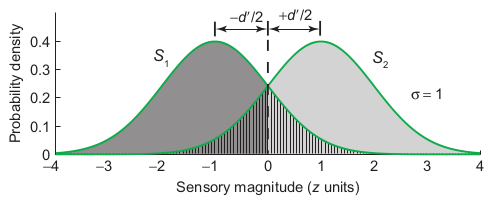
\includegraphics[scale=0.7]{../imagenes/modelosthurst.png}
			    \centering
			    \caption{Ejemplo de cálculo de d' utilizando modelos thursthonianos. Fte: \cite{PsychophysicsB} }
			    \label{fig:modelost}
            \end{figure}
            
            Además de lo ya expuesto, este tipo de análisis es especialmente interesante porque nos permite ordenar los valores obtenidos para $d'$ de forma que las diferencias entre ellos nos da información cuantitativa sobre cómo de diferentes o de similares son cada una de las distribuciones. Con la facilidad añadida que tiene este sistema para representar gráficamente mediante las técnicas habituales como diagramas de barras, entre otros.
            
\bibliography{biblio.bib}
\bibliographystyle{ieeetr}    
\end{document}